\documentclass[12pt]{article}
\usepackage{ctex}
\usepackage[a4paper, left=3cm, right=3cm, top=2.24cm, bottom=2.4cm]{geometry}
\usepackage[T1]{fontenc}
\usepackage{mathptmx}
\usepackage{amsmath}
\usepackage{indentfirst}

\usepackage[ruled,lined,commentsnumbered]{algorithm2e}
\usepackage{amsfonts}
\usepackage{chemformula}
\usepackage{indentfirst}
\usepackage{cite}
\usepackage{booktabs}
\usepackage{listings}
\usepackage[colorlinks, linkcolor=black, anchorcolor=blue, citecolor=black]{hyperref}
\usepackage{graphicx}
\usepackage{subfigure}


\usepackage{ulem}


\definecolor{mygreen}{rgb}{0,0.6,0}
\definecolor{mygray}{rgb}{0.5,0.5,0.5}
\setlength{\parskip}{0.5em}
\title{ 
	}

\author{\textup{\underline{林黄轩 ~ 毛钶翔 ~ 姚逸飞 ~ 郜尚 ~ 龚欣雨}}}
\renewcommand\contentsname{\LARGE\textsc{content}}
\lstset{
    basicstyle          =   \sffamily,          
    keywordstyle        =   \bfseries,          
    commentstyle        =   \rmfamily\itshape,  
    stringstyle         =   \ttfamily, 
    flexiblecolumns,                
    numbers             =   left,   
    showspaces          =   false,  
    numberstyle         =   \zihao{-5}\ttfamily,   
    showstringspaces    =   false,
    captionpos          =   t,     
    frame               =   none,
}

\lstdefinestyle{c++}{
    language        =   c++, % 语言选C++
    basicstyle      =   \zihao{-5}\ttfamily,
    numberstyle     =   \zihao{-5}\ttfamily,
    keywordstyle    =   \color{blue},
    keywordstyle    =   [2] \color{red},
	stringstyle     =   \color{magenta},
	backgroundcolor =   \color[RGB]{245,245,244},
    commentstyle    =   \color{mygreen}\ttfamily,
    breaklines      =   true,   % 自动换行,建议不要写太长的行
    columns         =   fixed,  % 如果不加这一句,字间距就不固定,很丑,必须加
	basewidth       =   0.5em,
}
\begin{document}
\begin{titlepage}
	\newcommand{\HRule}{\rule{\linewidth}{0.5mm}}
	
\includegraphics[width=8cm]{title/logo.png}\\[1.3cm] 
	\center 
	\quad\\[1.5cm]
	\textsl{\large School of Electrical Infomation and Electronic Engineering}\\[0.5cm] 
	\makeatletter
	\HRule \\[0.4cm]
	{ \huge \kaishu
	工科创IV-D Lab\_1 实验报告 \\ \Large 人机交互(HMI)综合实验 \@title}\\[0.4cm] 
	\HRule \\[1.5cm]


	\zihao{-3}\emph{第四组:} \@author
	
	
	
	\makeatother
	{\large  HMI Experiment for Science and Technology Innovation}\\[0.5cm]
	{\large \emph{Course Code: EI229}}\\[0.5cm]
	{\large \today}\\[2cm] 
	\vfill 
\end{titlepage}

\tableofcontents
\newpage

\section*{变量解释表}

\begin{table}[htbp]
	\centering
	\begin{tabular*}{16cm}{p{60pt}p{110pt}p{250pt}}
		\toprule
		变量名 & 作用域 & 变量作用 \\
		\midrule
		Var1 & 全局(任务1) & 作为时钟的递增信号\\
		Var2 & 全局(任务2) & 作为旋转编码开关控制的数字变量(QESVar)\\
		beepFlag & 全局(蜂鸣器控制)& 为避免主循环中使用delay导致计数延迟而使用的控制变量,用以判断蜂鸣器是否鸣响\\
		beepCnt & 全局(蜂鸣器控制) & 用作蜂鸣器鸣响时间的计数变量,在时间脉冲的中断中进行累加\\
		beepGap & 全局(蜂鸣器控制) & 控制蜂鸣器的鸣响时间($5ms * beepGap$)\\
		CountMAX & 全局(蜂鸣器控制)& 用以记录蜂鸣器鸣响的数值,该数值可更改\\
		sw1Flag & 全局(主循环) & 用以控制主循环中状态变化后的变量初始化,如果无需初始化可注释本部分代码\\
		initVar() & 子函数 & 初始化控制变量与计数变量,切换间隙会在LED屏幕上显示\emph{RESET},时间长短可变\\
		ResetFlag stopFlag & 全局(任务1) & 用以实现任务1功能且消除抖动的布尔值,分别在进入时和S2按下时生效\\

		QESPFlag & 全局(任务2) & 用以控制按下QES后的重置与防抖\\
		appTick appTick2 & 全局(时间中断) & 用以进行时间脉冲的中断计数\\
		INTF & 全局(QES中断) & 用以消除QES旋转时的抖动\\



		\bottomrule
	\end{tabular*}
\end{table}

\section{实验目标与问题整理}
\subsection{实验目标}


使用Cyber-Dorm K66单片机完成以下功能:
\begin{enumerate}
	\item 定义两个变量Var1、Var2,Var1初值0,Var2初值128
	
	\item 通过拨码开关SW1切换执行以下两个任务
	
	a) 程序主循环计数值显示及控制

    - S1按键(Key1)使Var1清零并开始主循环计数,S2按键停止计数

    - 主循环计数值达到某一个特定数值时蜂鸣器短鸣一声

    - 主循环计数值取0x0F的余数显示于数码管

    - 合理设置延时时长使显示字符清晰可见

    - 测试“反应能力”:听到蜂鸣器鸣叫后尽快按下S2,看计数值

  b) 数码开关QES变量显示及控制

    - QES顺时针旋转Var2数值增加,Var2最大值为十进制数255(0xFF)

    - QES逆时针旋转Var2数值减小,Var2最小值为0

    - 按下QES开关使Var2恢复初值128(0x80)

    - Var2数值显示于光柱或OLED
	\item S1、S2和数码开关的信号可能会出现“抖动”,通过程序处理实现简单的“防抖”功能。
\end{enumerate}

\subsection{问题整理}

根据小组掌握的知识,将上述目标整理为以下4个关键问题:

\begin{enumerate}
	\item 通过拨码开关切换不同的程序或执行不同的函数
	\item 计数逻辑与计数函数,延时参数调试,按键输入与OLED显示、数码管输出的应用
	\item 数码开关输入与液晶屏和光柱输出的应用
	\item 针对不同功能的信号特点设计对应的防抖算法
\end{enumerate}

\section{问题分析}


\subsection{工作程序的切换}

通过拨码开关SW1的输入,可以进行两个程序的切换。当拨码开关未被按下时,系统执行任务1;当开关被按下时,系统执行任务2。在任务状态变更后对原始变量进行重置(也可保留)。

\subsection{程序主循环数值显示及控制}

\subsubsection{功能实现}

在不同条件下通过按动按键来实现不同功能的任务容易使用分支语句配合辅助的布尔型变量来实现。计数功能通过单片机的计时器配合合理的延时函数来实现。

本试验采用八段共阳极数码管,用来显示一位数字 8 的七个笔画与 1 位小数点,所有发光二极管的阳极接到一起形成公共阳极的数码管,其在应用时应将公共极接到VCC上,当某一字段发光二极管的阴极为低电平时,相应字段就点亮,反之为高电平时,相应字段就不亮。显示功能通过\textbf{CDK66\_OLED}头文件中的函数以及\textbf{ShowNumHEX()}函数来实现。利用\textbf{BOARD\_I2C\_GPIO()}函数还可以实现光柱的数值显示控制。

\begin{figure}[htbp]
	\centering
	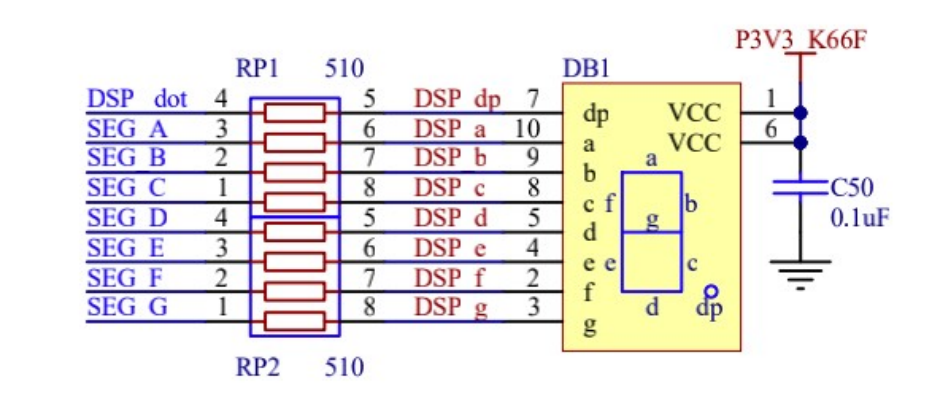
\includegraphics[width = 0.8\textwidth]{graph/pic1.png}
	\caption{八段共阳极数码管原理图}
\end{figure}

\subsubsection{防抖方法}

按键按动过程中,由于机械上的振动或电位上的不稳定,产生的信号会带有一定的跳动,而单片机的识别周期极短,可以检测到这些跳动从而产生误判,防抖的基本原理就是让通过程序滤除这些跳动。在本实验中,我们通过标志位的状态变化来实现软件防抖操作,降低程序对于延时的需求。在案件按下后,标志位拉起,直到按钮弹起后再置零。同时使用全局变量控制不会干扰其他工作的正常执行,使得按下按钮时可同时进行其他操作。

\subsection{数码开关QES变量显示及控制}
\subsubsection{功能实现}

该任务要求的功能较为简单,通过例程中定义好的\textbf{QESB()、QESA()和QESP()}函数,结合正交信号的原理容易设计函数实现拨码盘控制变量Var2增减的功能。

本实验采用的旋转编码开关,采用正交编码的方式,通过判断高低电平可以读取旋转方向。若采取 A 信号上升沿时调用程序,则通过在中断服务程序中读取的B信号的状态,可知B为高电平,说明为正转。反之,当B为低电平时,说明为反转。旋转编码开关的原理如下图所示:
\begin{figure}[htbp]
	\centering
	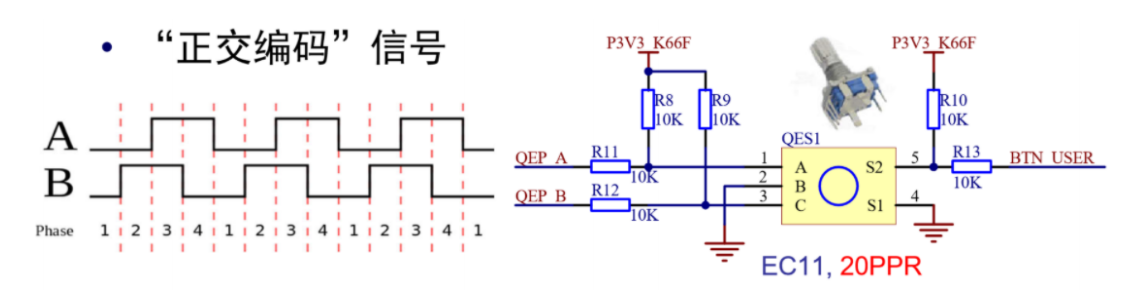
\includegraphics[width = \textwidth]{graph/pic2.png}
	\caption{旋转编码开关原理图}
\end{figure}

\subsubsection{防抖方法}
由于编码盘使用正交编码,可发现在A相的上升沿与下降沿之间会发生B相的转换,任何一相在正常情况下不会发生连续的变换。因此需要确认读取B相状态时A相应处于上升沿触发后、下降沿触发前。最为合理的防抖方法是配置A相与B项的双中断,仅当读取到两个不同的中断后再进行状态变化。但程序使用的中断配置有限,无需为此多添加一个中断串口,所以我们通过对A的上升沿与下降沿两侧的中断监控进行防抖处理。

A相出现漂移时可能会导致短时间多次触发上升沿中断,这也是抖动的主要原因。我们设置A相上升沿中断标志位\textbf{INTF},在下降沿触发时再将其置零,防止连续的状态变化。这样可以避免在中断中使用长时间的delay导致中断持续被占用,提高程序的运行效率。

\begin{figure}[htbp]
	\centering
	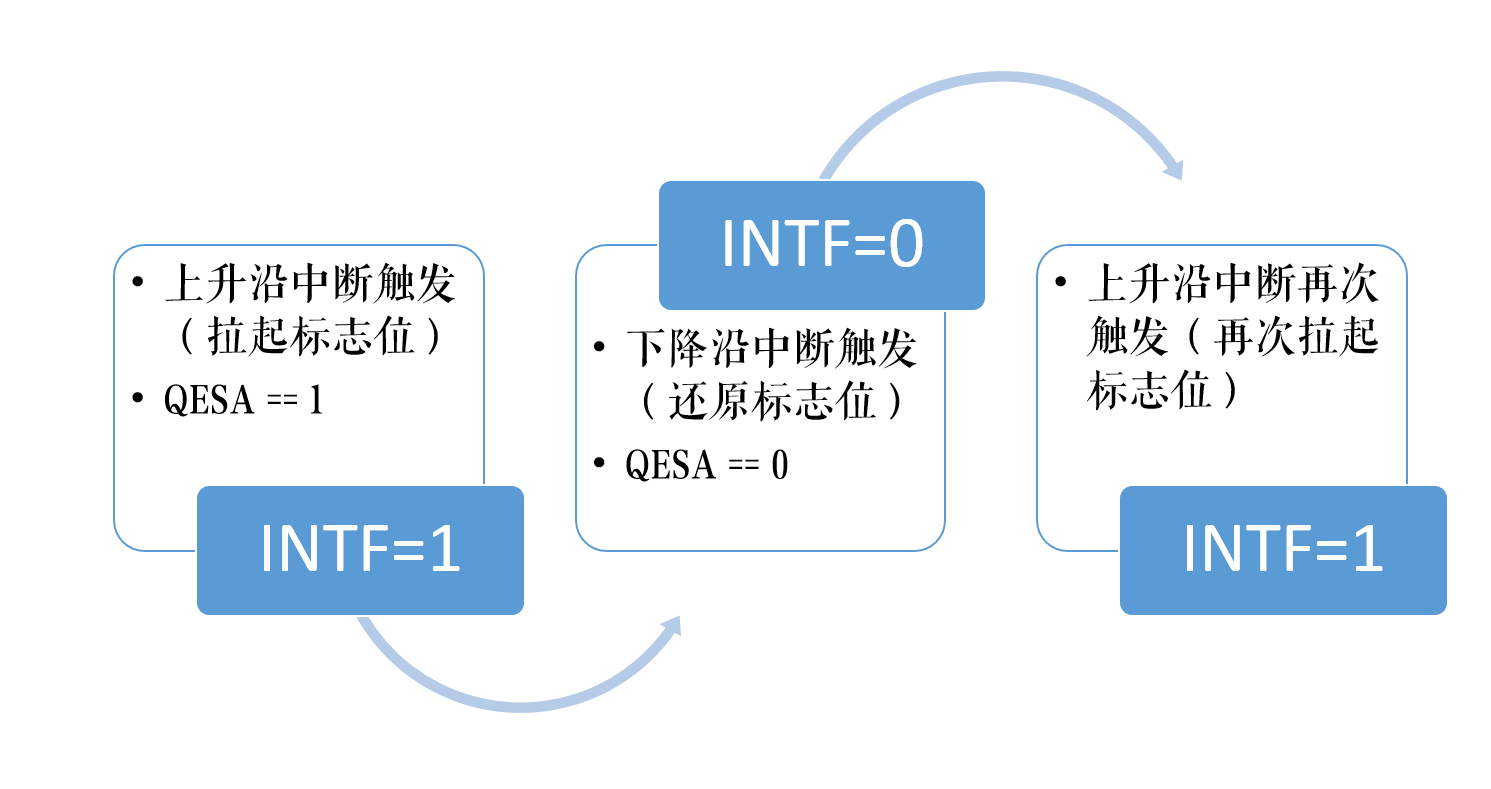
\includegraphics[width = 0.8\textwidth]{graph/form.png}
	\caption{防抖实现原理示意图}
	\label{pic:prin}
\end{figure}

\section{程序开发}
\subsection{任务1代码实现}

\subsubsection{程序主体}

程序主体部分代码如下所示
\lstinputlisting[
style       =   c++,
caption     =   {\bf void Task1},
label       =   {code:task1}
]{code/1.c}

代码禁用了OLED屏幕与光柱,其中5$\sim$16行使用\textbf{ResetFlag}标识符进行S1的抖动消除,而17$\sim$25行则实现了S2的抖动消除。二者均在弹起后进行重置,并通过全局变量保证了标识符在不同循环中的传输。26$\sim$34行实现了\textbf{Var1}的按秒递增,并通过\textbf{while循环检测appTick2的变化}以实现准确的秒控制。程序在主体中执行蜂鸣器的鸣响并挂起鸣响标志,在鸣响的瞬间按下S2可终止蜂鸣器鸣响,用以模拟闹钟功能。如不进行重置,则蜂鸣器会在鸣响一定时间后停止。

代码第29行实现了数字在八位数码管上的显示,通过调用\textbf{ShowNumHex}函数显示16进制的最低位数字。单个数值显示时间为1秒。
\subsubsection{中断处理}

中断处理部分代码如下所示
\lstinputlisting[
style       =   c++,
caption     =   {\bf Task 1中断处理},
label       =   {code:int1}
]{code/2.c}

在时钟信号的基础中断中,我们加入了鸣响标识符被挂起的判断。鸣响标志\textbf{BeepFlag}在\autoref{code:task1}中被挂起并启动中断中的蜂鸣器计时。在蜂鸣器鸣响达到指定时间后终止计时、置零标识符并关闭蜂鸣器。

\subsection{任务2代码实现}

\subsubsection{程序主体}

任务2的程序主体部分如下所示
\lstinputlisting[
style       =   c++,
caption     =   {\bf Task2},
label       =   {code:task2}
]{code/3.c}

程序主体主要实现了旋转编码开关按下后对Var2的初始化,通过QESPFlag实现对这一进程的控制与防抖。同时通过\textbf{OLED\_Print\_Num函数和BOARD\_I2C\_GPIO函数}使得Var2变量可以输出到OLED显示屏和光柱。

\subsubsection{中断处理}

任务2中断处理部分如下所示
\lstinputlisting[
style       =   c++,
caption     =   {\bf Task2中断处理},
label       =   {code:int2}
]{code/4.c}

这一中断使用A相的上升沿与下降沿触发,因此需要在pin->路由详情中配置99号对应的QESa触发方式为\emph{interrupt on either edge}。

代码分别判断上升沿中断与下降沿中断的情况。当上升沿触发后,QESA()读取到高电平,此时判断上升沿的操作是否被访问过,如果被访问过则直接跳过以消除抖动,如果没有被访问过则进入条件并依据B相的状况改变Var2的数值。
当下降沿触发后,QESA()读取到低电平,此时访问上升沿的次数被清零,可以执行下一次变化。具体执行流程可以参考图\ref{pic:prin}。

由于Var2的最大值为255,程序中对其执行模运算并保留模256的余数。


\subsection{任务切换与重置}
任务切换的判断在主程序的while循环中执行,其代码如下:
\lstinputlisting[
style       =   c++,
caption     =   {\bf 主函数while循环},
label       =   {code:while}
]{code/5.c}

程序通过标识符实现状态的切换与重置。切换时只需监督判断SW1的状态,如果其读数为1则执行Task1,反之则执行Task2。
通过SW1Flag可以判断状态是否发生变化。如果发生变化则对变量进行初始化。由于两个任务的变量不相关,所以在两次切换中只需执行一次初始化。

对于初始化代码,我们添加了一些特殊功能,具体代码如下:
\lstinputlisting[
style       =   c++,
caption     =   {\bf 初始化},
label       =   {code:init}
]{code/6.c}

在变量初始化的过程中,我们让OLED屏幕输入一段时间的“RESET”,表示其正在执行代码的初始化\footnote{其实代码的执行非常短暂,但是我们想让这一过程看上去更有仪式感}。

\section{实验结果}

\subsection{使用拨码开关SW1切换任务}
\begin{figure*}[htbp]
	\centering
	\subfigure[按下开关前]{\rotatebox{90}{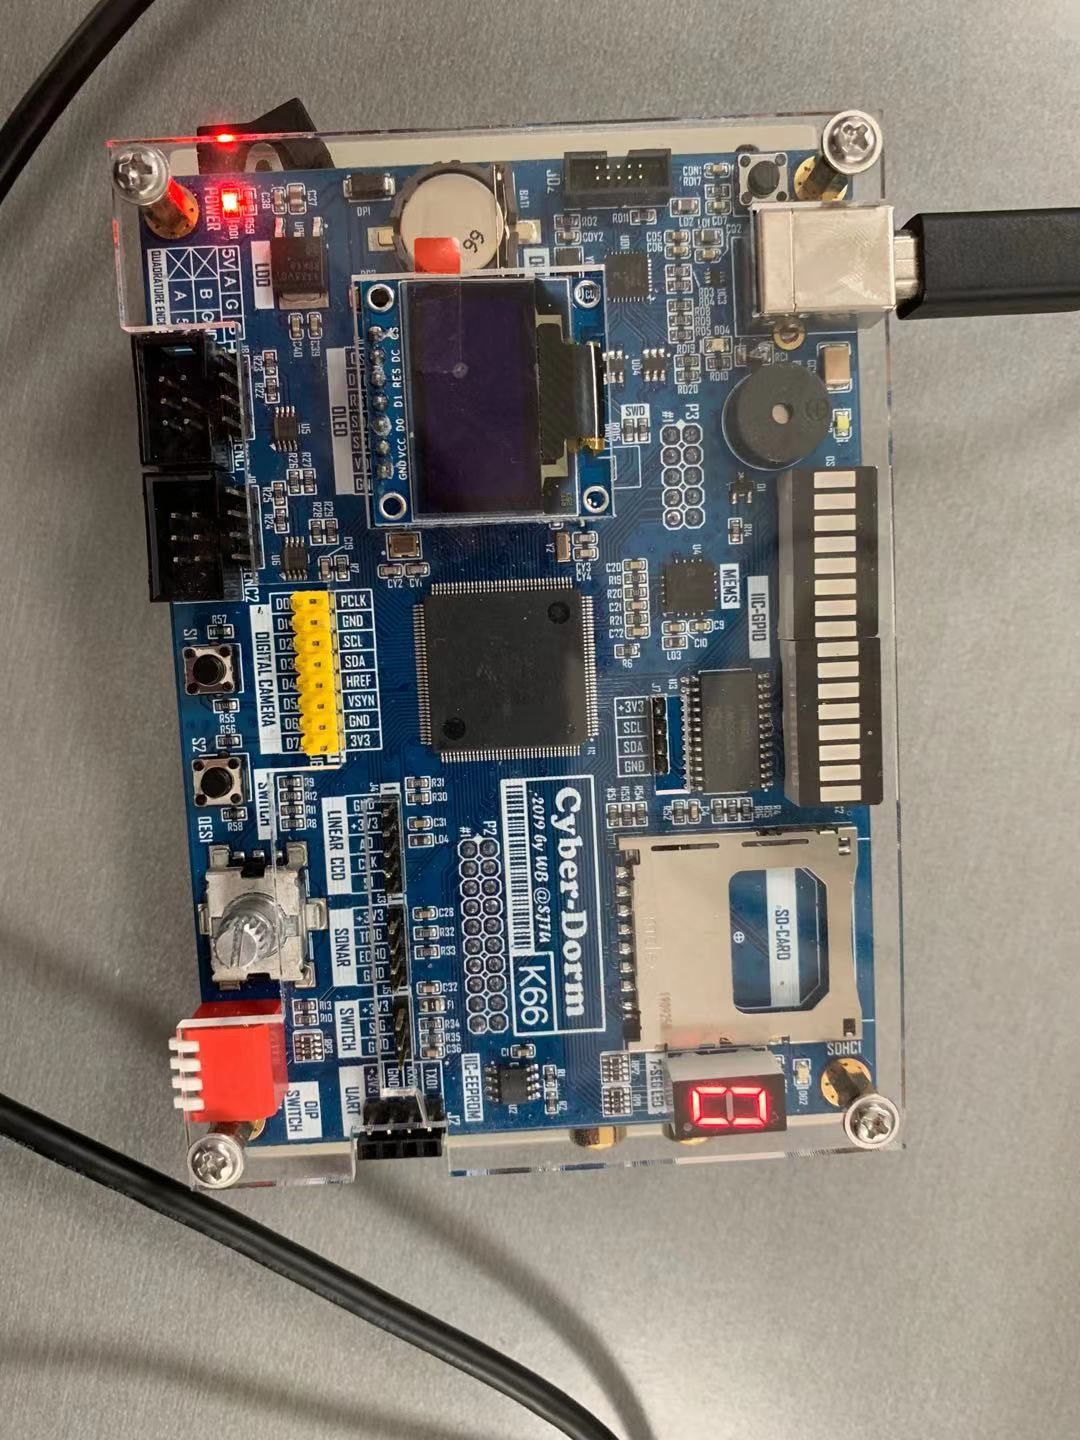
\includegraphics[width=0.3\textwidth]{graph/1-1.jpg}}}
	\subfigure[按下开关后]{\rotatebox{90}{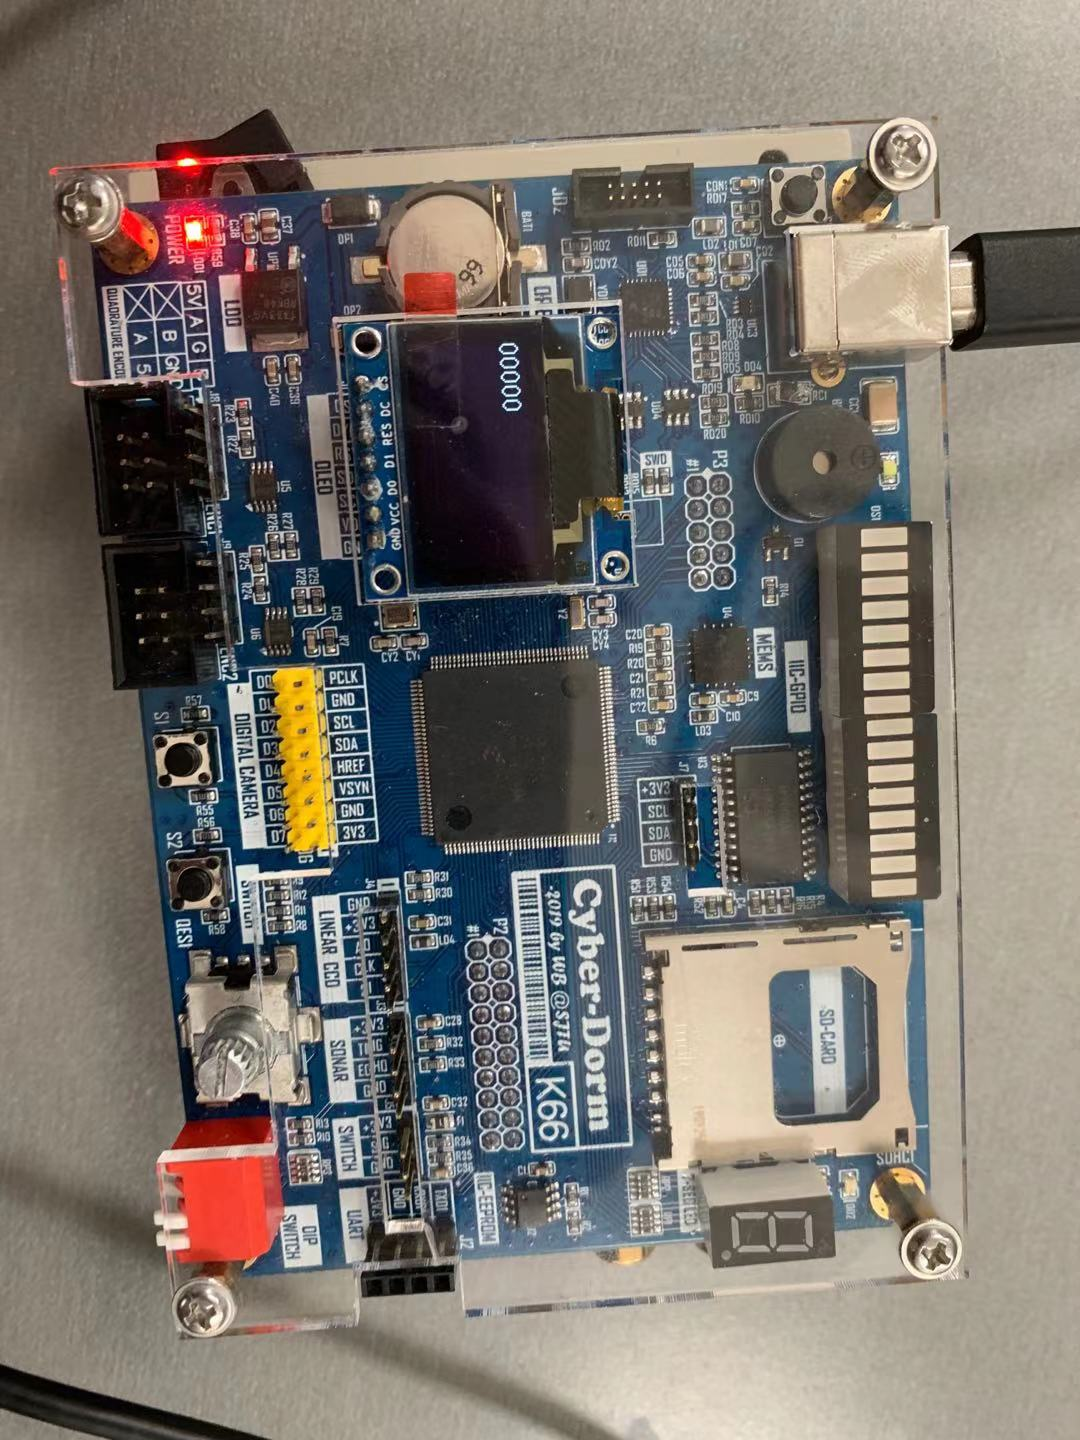
\includegraphics[width=0.3\textwidth]{graph/1-2.jpg}}}
	
\end{figure*}

\subsection{任务1的执行}

\begin{figure*}[htbp]
	\centering
	\subfigure[显示余数为0]{\rotatebox{90}{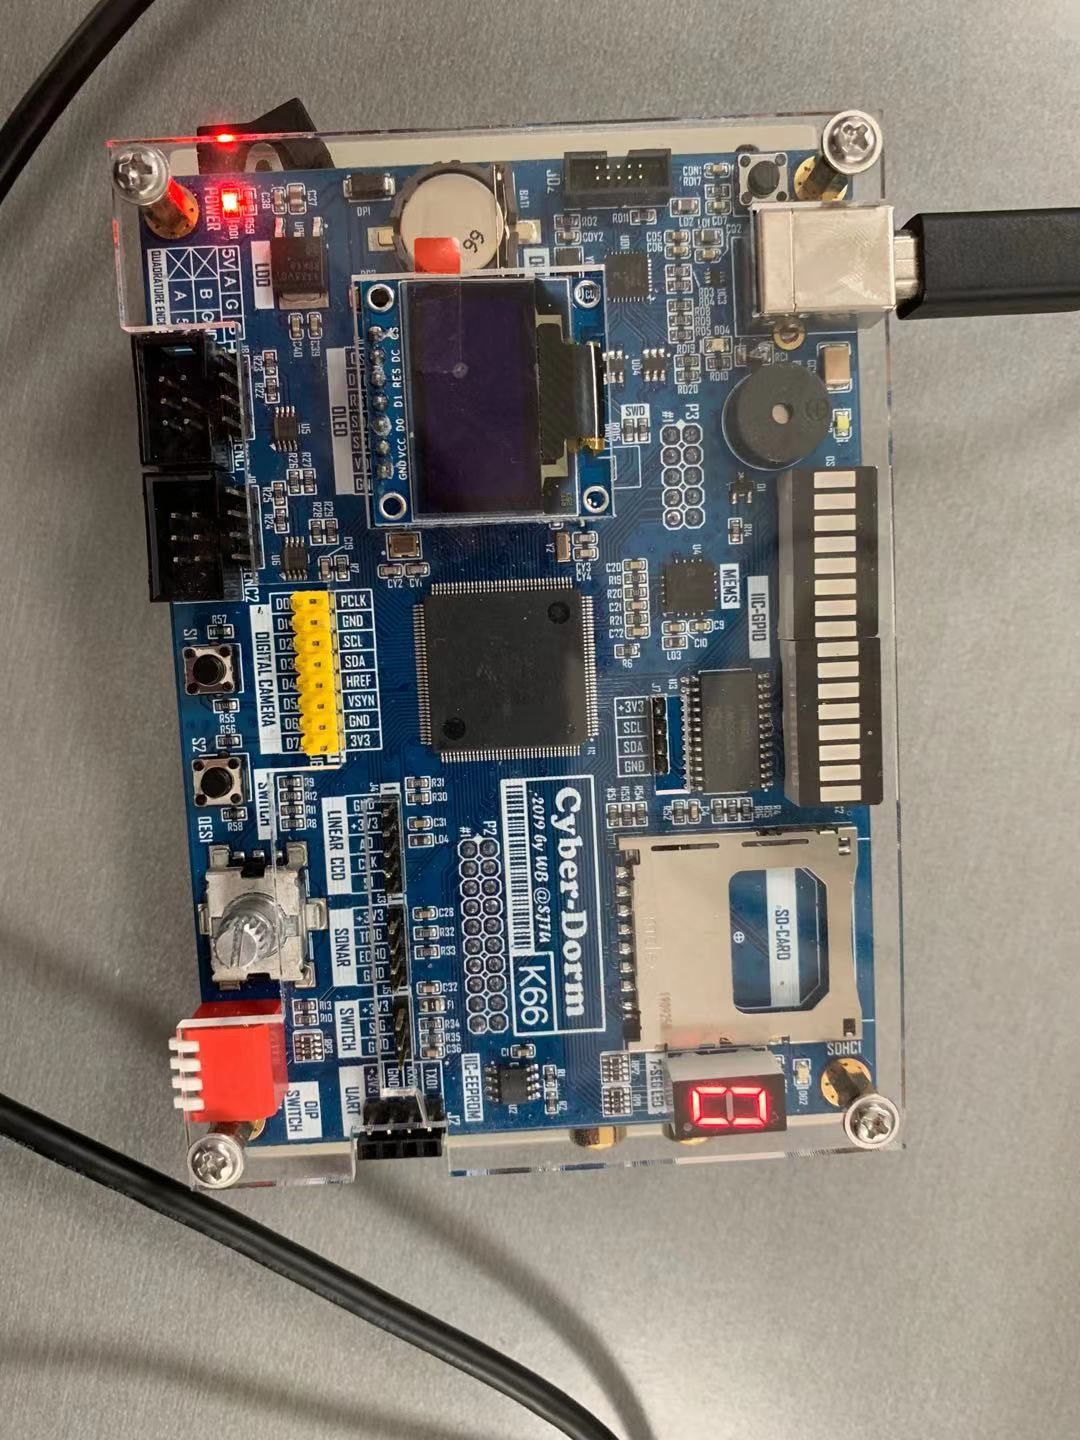
\includegraphics[width=0.3\textwidth]{graph/1-1.jpg}}}
	\subfigure[显示余数为E]{\rotatebox{90}{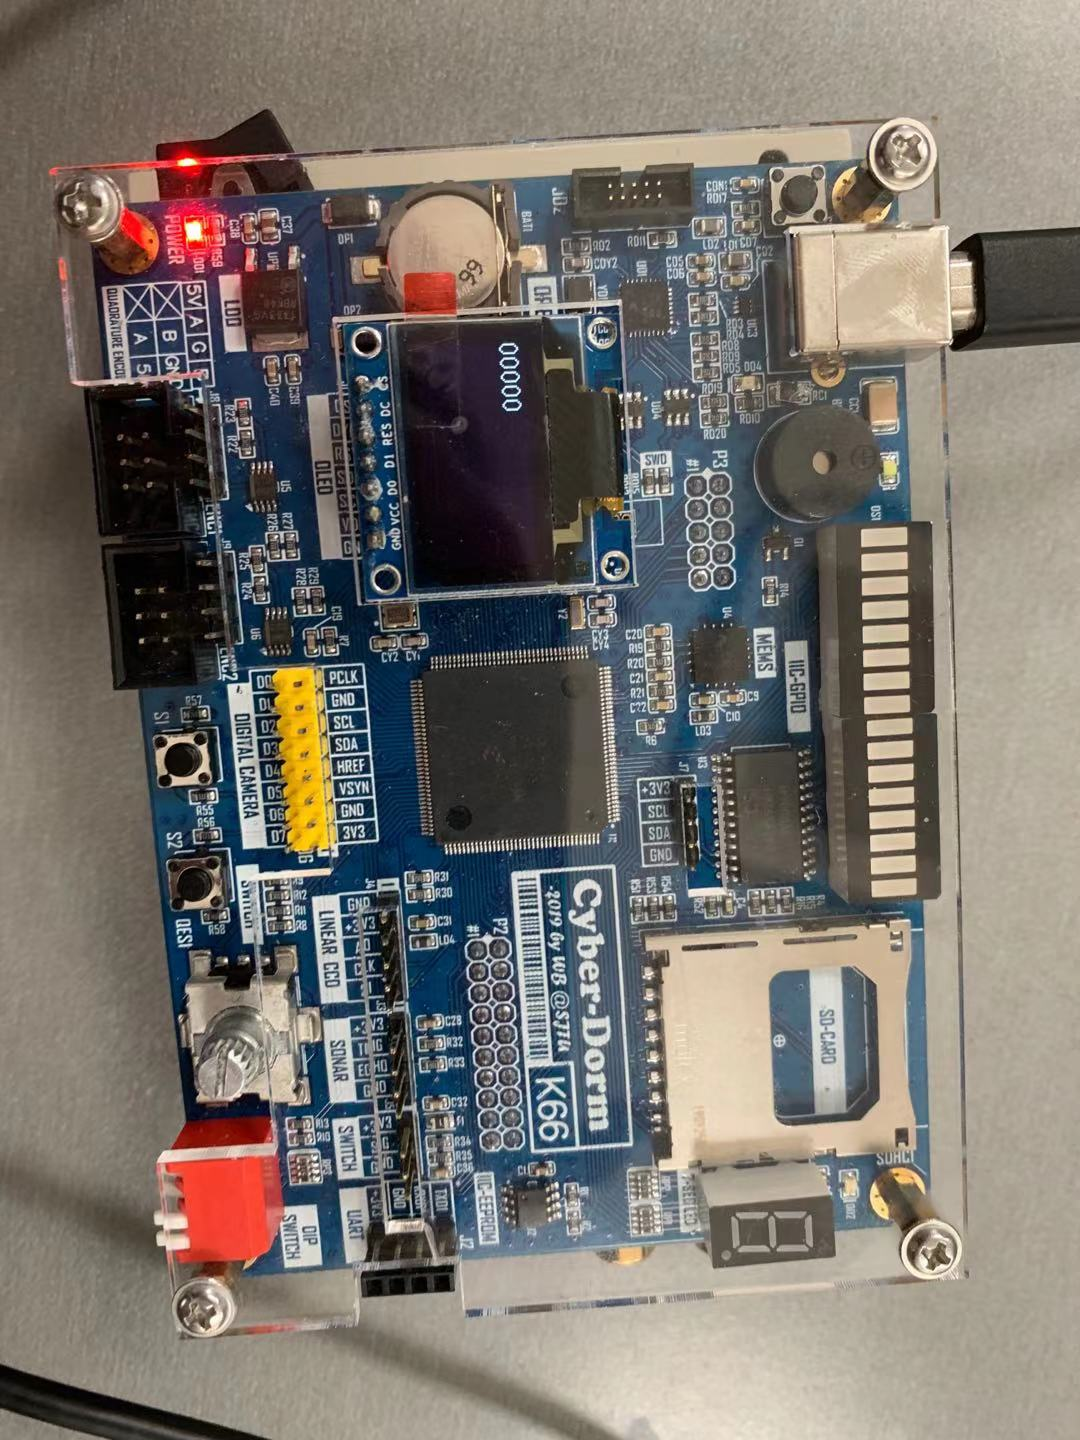
\includegraphics[width=0.3\textwidth]{graph/1-3.jpg}}}
	
\end{figure*}

在合理设置延时时长后,可以顺利完成计数、暂停、启动、置零和特定数值提示并计数的功能,并可以清楚地观察到Var1变量的每次变化。按下S2后,计时停止;按下S1后,计时清零。以上内容连续进行20次操作未出现因抖动问题而产生的异常情况。

\subsection{任务2的执行}
\begin{figure*}[htbp]
	\centering
	\subfigure[Var2为0]{\rotatebox{90}{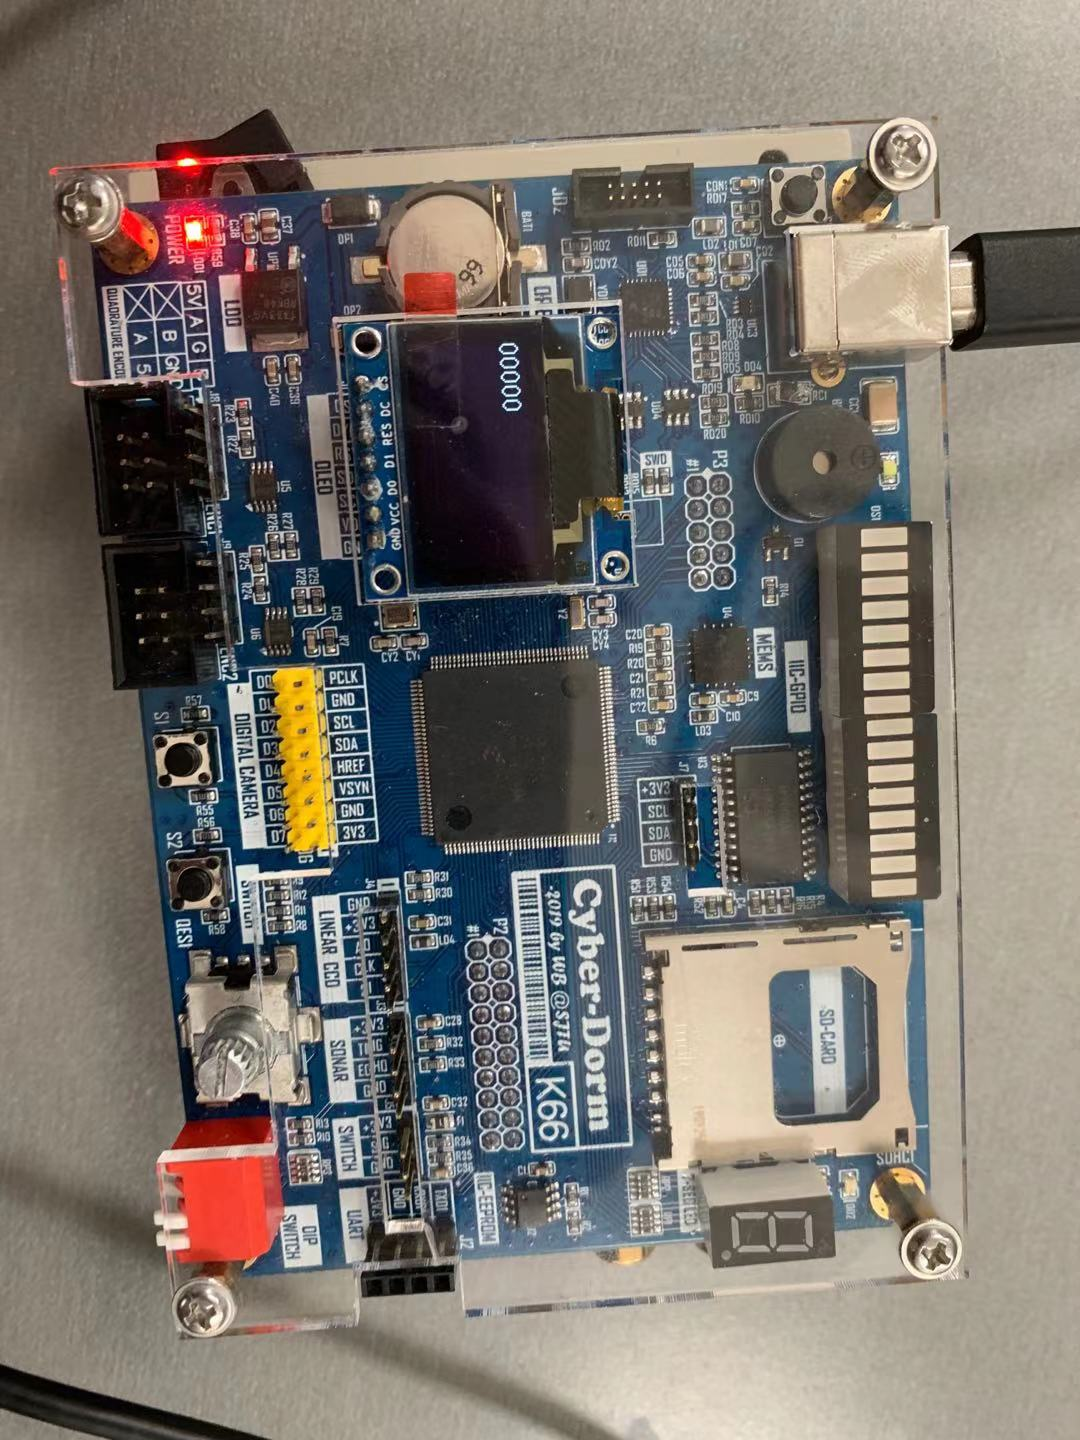
\includegraphics[width=0.3\textwidth]{graph/1-2.jpg}}}
	\subfigure[Var2为128]{\rotatebox{90}{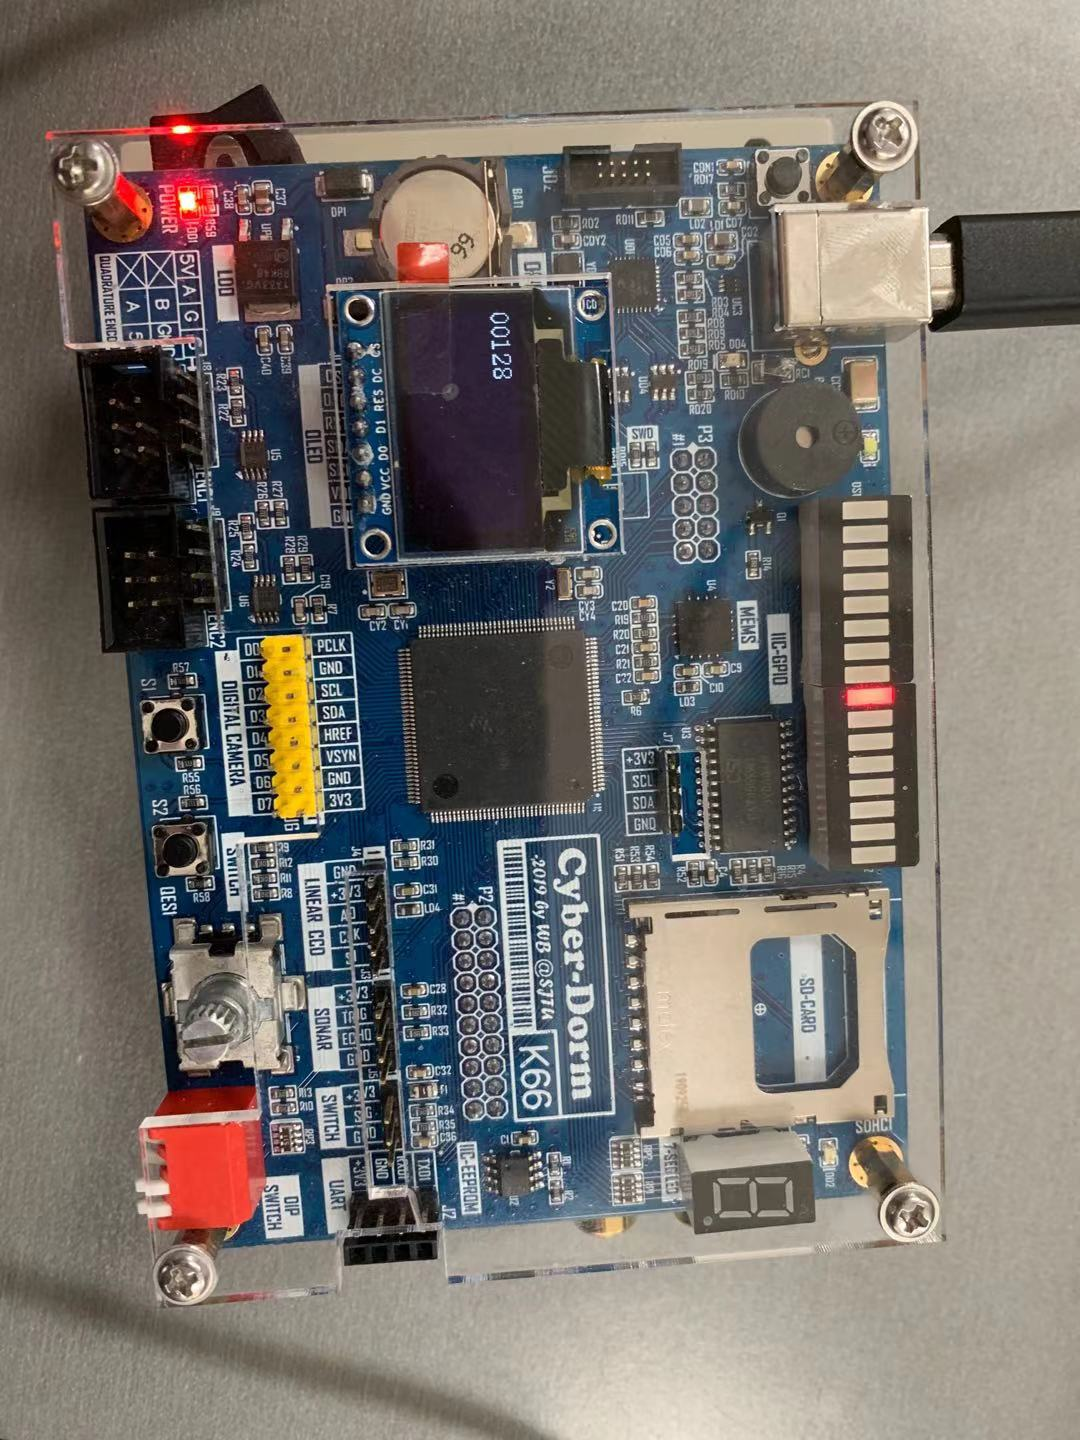
\includegraphics[width=0.3\textwidth]{graph/1-4.jpg}}}
	\centering
	\subfigure[Var2为255]{\rotatebox{90}{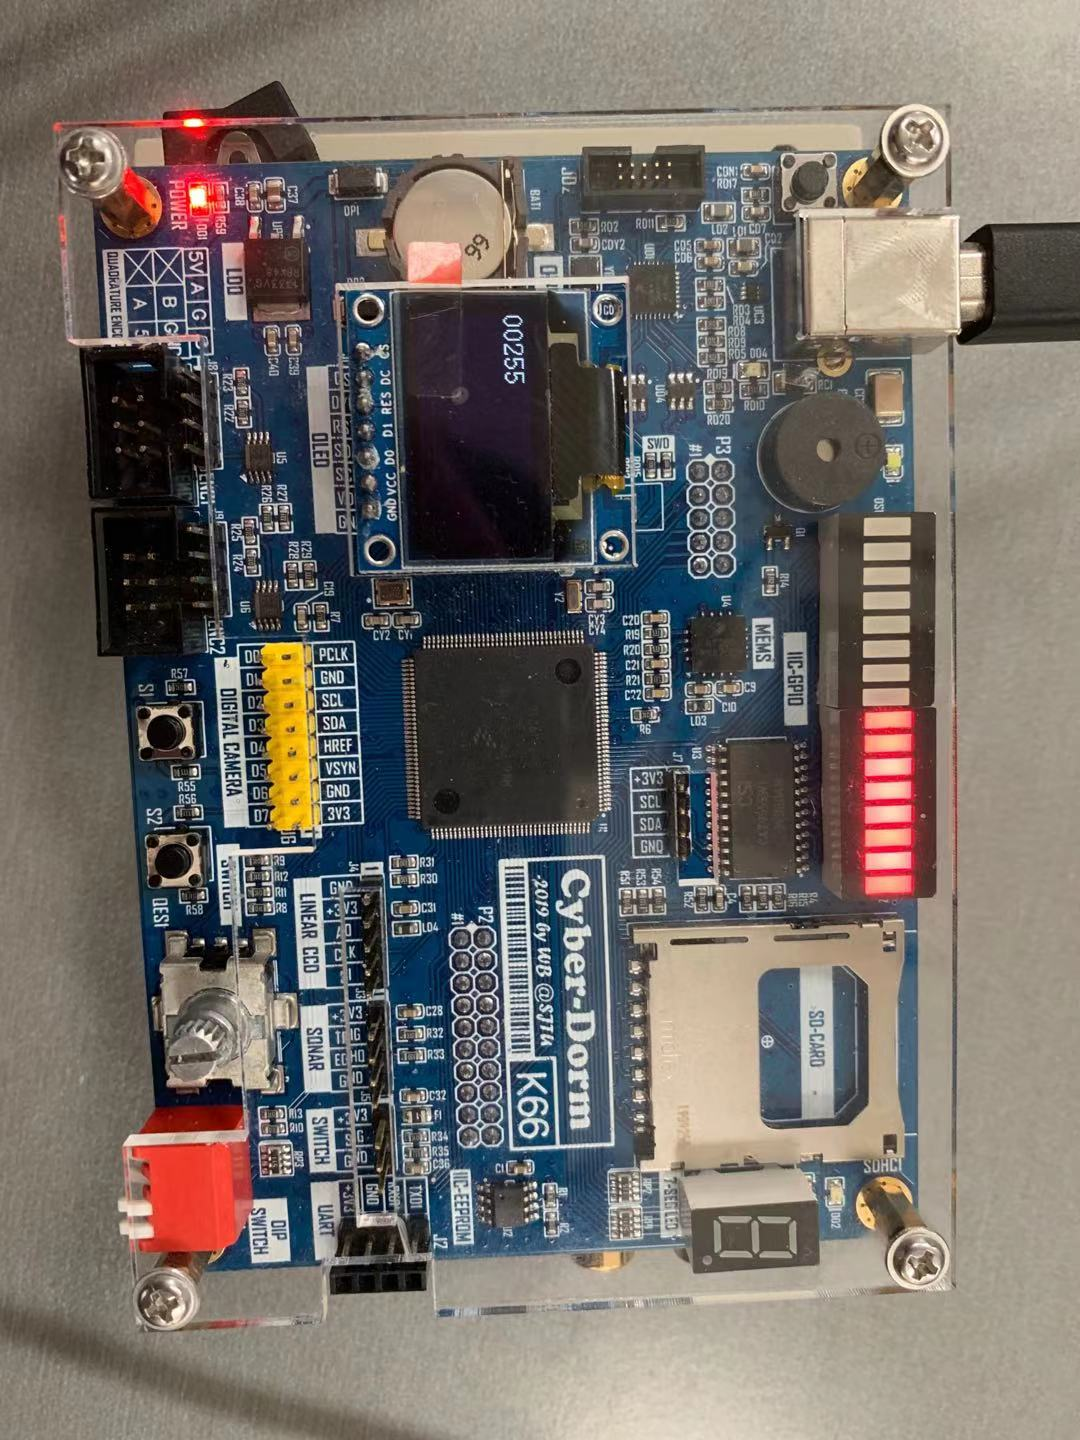
\includegraphics[width=0.3\textwidth]{graph/1-5.jpg}}}
\end{figure*}

使用双侧中断判定的方法,实验验证可以起到较好的防抖效果,连续拨动拨码盘使Var2从128经过255回到128,再进行逆向操作,最后按动数码拨盘使Var2回复128再重复一遍该过程,测试过程中未出现因抖动问题而产生的参数异常变化。

通过光柱的变化可以观察当拨码盘快速旋转时Var2的变化。可以发现其变化是连续的,说明在转动过程中没有受到抖动影响,无论速度快与否。

\section{结论}

在本次实验中,小组成员分工明确,互帮互助,共同熟悉了基于Cyber-Dorm K66单片机的简单人机交互开发,进一步了解了拨码开关、按键、拨码盘、OLED屏幕、八段数码管等基本元器件的使用原理并基于不同的信号原理设计了对应的防抖函数。

在任务一中,小组结合课堂学习中有关按键开关的知识,配合板载时钟利用分支语句和布尔变量\footnote{C语言不存在bool的关键字,这里使用字符类型uint8\_t来模拟其效果}完成了程序的编写。该任务进一步提高了小组成员阅读和理解代码框架并加以应用的能力。

任务二中,小组成员学习了旋转拨码开关的工作原理和中断触发机制,完成了功能的实现,姚逸飞同学富有创见地提出了双边沿中断判定的方法实现并编写了相应的防抖代码,取得了较好的实际效果。小组成员在该实验中互相交流,更加深入地理解了防抖代码的编写思想和应用。


\end{document}